\subsection{Existing Products and Projects}
% how have other projects and products used similar strategies to FORWARD?

\noindent There have been numerous efforts made by researchers to develop smart walkers using the available technologies. Perhaps the seminal work in this growing field of research and development is \cite{PAMM}. This group was the first to propose a smart walker project with localization, mobility control, and object avoidance. In the following sections we seek to analyze these technologies and methods in a way that identifies which of such will be most desired for our specific system, taking into consideration many factors, some of which being: cost, attainability, integration complexity, and performance.

%% Toby research here
\subsubsection{Current Walker Sensing Applications}
\noindent In the smart walker prototype created in \cite{Mostofa}, nine HC-SR04 ultrasonic sensors are arrayed along the front of the walker. Seven face forward, while the remaining two point perpendicularly to the walker motion and opposite to each other. This setup provides a continuous reading of the walker's forward hemisphere with a detection range of 200cm. Our team asks the question, can obstacle detection and notification be achieved with a more discrete array of sensors stowed onto the walker frame? What is the operational FOV for ultrasonic sensors? Can the amount be reduced? How will the introduction of LiDAR and camera technology affect the ultrasonic approach?\\

\begin{figure}[h]
	\centering
	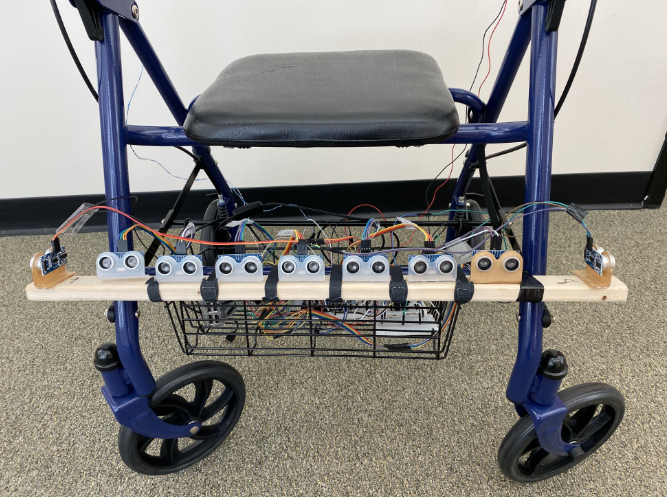
\includegraphics[width=0.5\textwidth]{./Images/mostafa9.png}
	\caption{\label{fig:mostafa9}"Rollator" with nine HC-SR04 sensors \cite{Mostofa}}
\end{figure}

\noindent Robotics are a popular use of LiDAR, often able to achieve feats such as autonomous delivery. However, many researchers have also introduced laser sensing methods and other waves near infrared in order to provide ranging data to mobile systems, which in our case is the walker. A senior design group at Michigan State University expanded on this \cite{mstate}.\\

\noindent In \cite{FallDetect}, the group implements one of FORWARD's stretch features with an unorthodox yet clever utilization of LiDAR and sensor fusion. In order to equip the walker with fall detection, both ultrasonic and laser sensors are installed near the footstep bay of the walker. They also add force sensors in the handlebars. The feedback provided by the sensing system is whether the user is walking uprightly. If the user began to fall, the laser sensors would reflect their feet moving out of view, and likely the force sensors would experience more pressure as the user reacted to a slip. \\

\noindent This walker does not employ GPS. We are not looking to track the location continuously. This technology has more of a place within the application of health monitoring and emergency alerts.\\


%% Matthew Research Here
\subsubsection{Existing Computer Vision/AI Image Processing Models}
 \underline{\textit{Ultralytics YOLO}} (You only look once) is an open source AI driven image processing model. The Ultralytics YOLO platform provides an AI Image processing Architecture that is malleable to the users demands, and for our case, would process the input image to detect if one of the five hazards is present, as well as provide a confidence rating for these predictions. To implement the object detection functionality to our specifications, minimal training, as well as coding must be performed. The benefits of this solution for our image classification system include zero cost and easy configurability which are both important aspects for our desired solution. The negatives include the needed man hours to train and implement this model for our purposes and time to run (anywhere from 0.1 seconds to 3 seconds). It also has a relatively high memory footprint (a few hundred MB). The time to predict along with the memory footprint could potentially exclude this from our options as we need to have classification under 1 second latency, ideally in the realm of a few hundred milliseconds and enough storage space for the model. \\
%https://www.freecodecamp.org/news/how-to-detect-objects-in-images-using-yolov8/#heading-how-to-get-started-with-yolov8 

\noindent \underline{\textit{FOMO}} (Faster objects, More objects) is a machine learning image processing algorithm that seeks to solve the problem of running high complexity algorithms (such as neural networks) on MCU's. In the documents referenced [HERE], the Arduino Nicla board is used to classify the objects in frame at a rate of 33 microseconds (30 SPS). The objects can be classified and processed through multiple methods, but all of which would be applicable to our purposes. This system also minimizes the memory usage by needing only 256 KB of memory to run and store these algorithms. On the FOMO website, they claim that this algorithm is compatible with many of the MCU's that we are considering for this project, some of which being an ESP32, Arduino Nicla, Raspberry Pi, and others. \\
%https://www.hackster.io/mjrobot/tinyml-made-easy-object-detection-with-nicla-vision-407ddd
%https://docs.edgeimpulse.com/docs/edge-impulse-studio/learning-blocks/object-detection/fomo-object-detection-for-constrained-devices

\noindent \underline{\textit{Spatial AI}} is the combination of both Visual AI and Depth AI, in tandem to identify objects for classification as well as identifying depth of objects for better guidance and classification. [Research the models that make this possible]\\
%https://learnopencv.com/object-detection-with-depth-measurement-with-oak-d/

\subsubsection{Existing Camera Technologies}
\noindent \underline{\textit{ESP 32 CAM Board}} is a ESP32 processor based camera module that can transmit video data at high resolutions, which can be processed by our CV/Image processing solution. The module also has WIFI connectivity that can connect to an MCU to wirelessly transmit the video stream. The module has a 32-bit CPU with a max clock frequency of 240 MHz and 520 KB of built-in SRAM with an external 4MB PSRAM. The board module also runs on FreeRTOS. The included camera, OV2640 camera, has a 2 MP resolution, up to 1600 x 1200 and interfaces the controller board over a 24 pin interface bus. A more advanced sister product to the OV2640 is the OV5640 camera. This camera has 5 MP resolution, up to 2592 x 1944. In order to achieve our stretch requirement of depth perception analysis for guidance and navigation, this camera could be advantageous.\\
%https://how2electronics.com/esp32-cam-based-object-detection-identification-with-opencv/
%https://how2electronics.com/getting-started-with-esp32-cam-board-video-streaming-over-wifi/

\noindent \underline{\textit{The Oak-D Lite}} camera is an AI robotics specific camera, capable of running AI models such as open CV. The camera is able to run on-board AI architectures to achieve object classification, edge detection, and feature tracking. This technology allow for high accuracy with object detection, and introduce the ability to implement edge detection as a means to depth perception, which can be used for routing in our GNC subsystem. The Oak-D Lite has a 13 MP RGB camera with auto-focus, as well a 60axis sensor using an accelerometer and gyroscope. It also uses USB2 and USB3 for power and communication, which is simple to interface to a RaspberryPI. The camera can run 4K at 30 FPS or 1080P at 60 FPS.\\


\subsubsection{Existing MCU Technologies}

\noindent 


%% Morgan Research Here
\subsubsection{Motor and Steering Applications} 

